\section{Introduction}\label{sec:intro}
\subsection{What it can do}\label{sec:intro:intro}
This package provides commands and syntaxes to help you draw musical notations in 
a \LaTeX\ document, based on the \tikzname\ package. You can see next page of 
this manual for a demo of it.

Note that this package is still \emph{very} experimental.
\subsection{Current limitations}\label{sec:intro:limitations}
Although the syntaxes are quite human-readable, they are very \emph{long}. In 
the future an easy-to-use front-end is necessary and should be implemented.

The speed is also an issue, as it requires time to draw many complex notations. 
For instance, the treble clef, |tm-g-clef|, takes $0.03$ seconds (in my machine) 
alone.\footnote{Thanks to the \pkg{l3benchmark} package.} The first page of 
\emph{F\"ur Elise}, displayed on the next page, takes about $10$ seconds for each 
PDF\LaTeX\ run. This has no easy fix though, as efficiency and beauty, in these 
cases, can't live under the same roof. If you need high speed, you can 
externalize your sheet music and include them as PDFs in your document.

There are many notations which are so advanced that I can't be confident enough 
to add them to the package. If you need them, feel free to submit a feature 
request to the \href{https://github.com/joulev/tikzmusic}{package repository}. 

Also, this documentation is written somewhat hastily, and may contain grammar 
mistakes from a non-native speaker. If you find typos or errors in the manual, 
feel free to send me a bug report.
\subsection{Thanks}\label{sec:intro:thanks}
First of all, I would like to thank the following people who have greatly 
helped me in writing this package:

\begin{itemize}
  % JouleV: I know this is an odd way to color hyperref, but anyway...
  \let\oldhref\href
  \def\href#1#2{\declare{\oldhref{#1}{#2}}}
  \item Till Tantau and every developer of the \tikzname-\pgfname\ package. 
  Obviously, without the powerful \pgfname\ and its easy-to-use front-end 
  \tikzname, this package, along with many others, would not be possible.
  \item The development team of all packages used by this package.
  \item Every member of the 
  \href{https://chat.stackoverflow.com/rooms/193903/duck-overflow}{Duck Overflow} 
  chat room and the \href{https://topanswers.xyz/tex}{Top\TeX} community, most 
  notably (but not limited to) marmot, samcarter and Skillmon, for their great 
  help in writing this package. My knowledge in \TeX\ and friends would not be 
  the same without these people.
  \item Christian Feuers\"anger for the |pgfmanual| documentation style, most 
  notably the automatic hyperlink in the documentation. The style was adopted 
  in the documentation of this package.
  \item The \href{https://inkscape.org/}{Inkscape} project and the 
  \href{https://github.com/kjellmf/svg2tikz}{\pkg{svg2tikz}} project. I have used these 
  two tools heavily to generate code for the musical notations from existing 
  SVG files. Although the files in {\sffamily tex/latex/tikzmusic/src/tm-paths} are 
  not automatically generated, most parts of them are generated by these tools.
  \item The \href{https://musescore.org}{MuseScore} project. Although I had known 
  some about music notations, that was too little for the package. I have used 
  MuseScore heavily for some ideas about music writing and music notations.
\end{itemize}

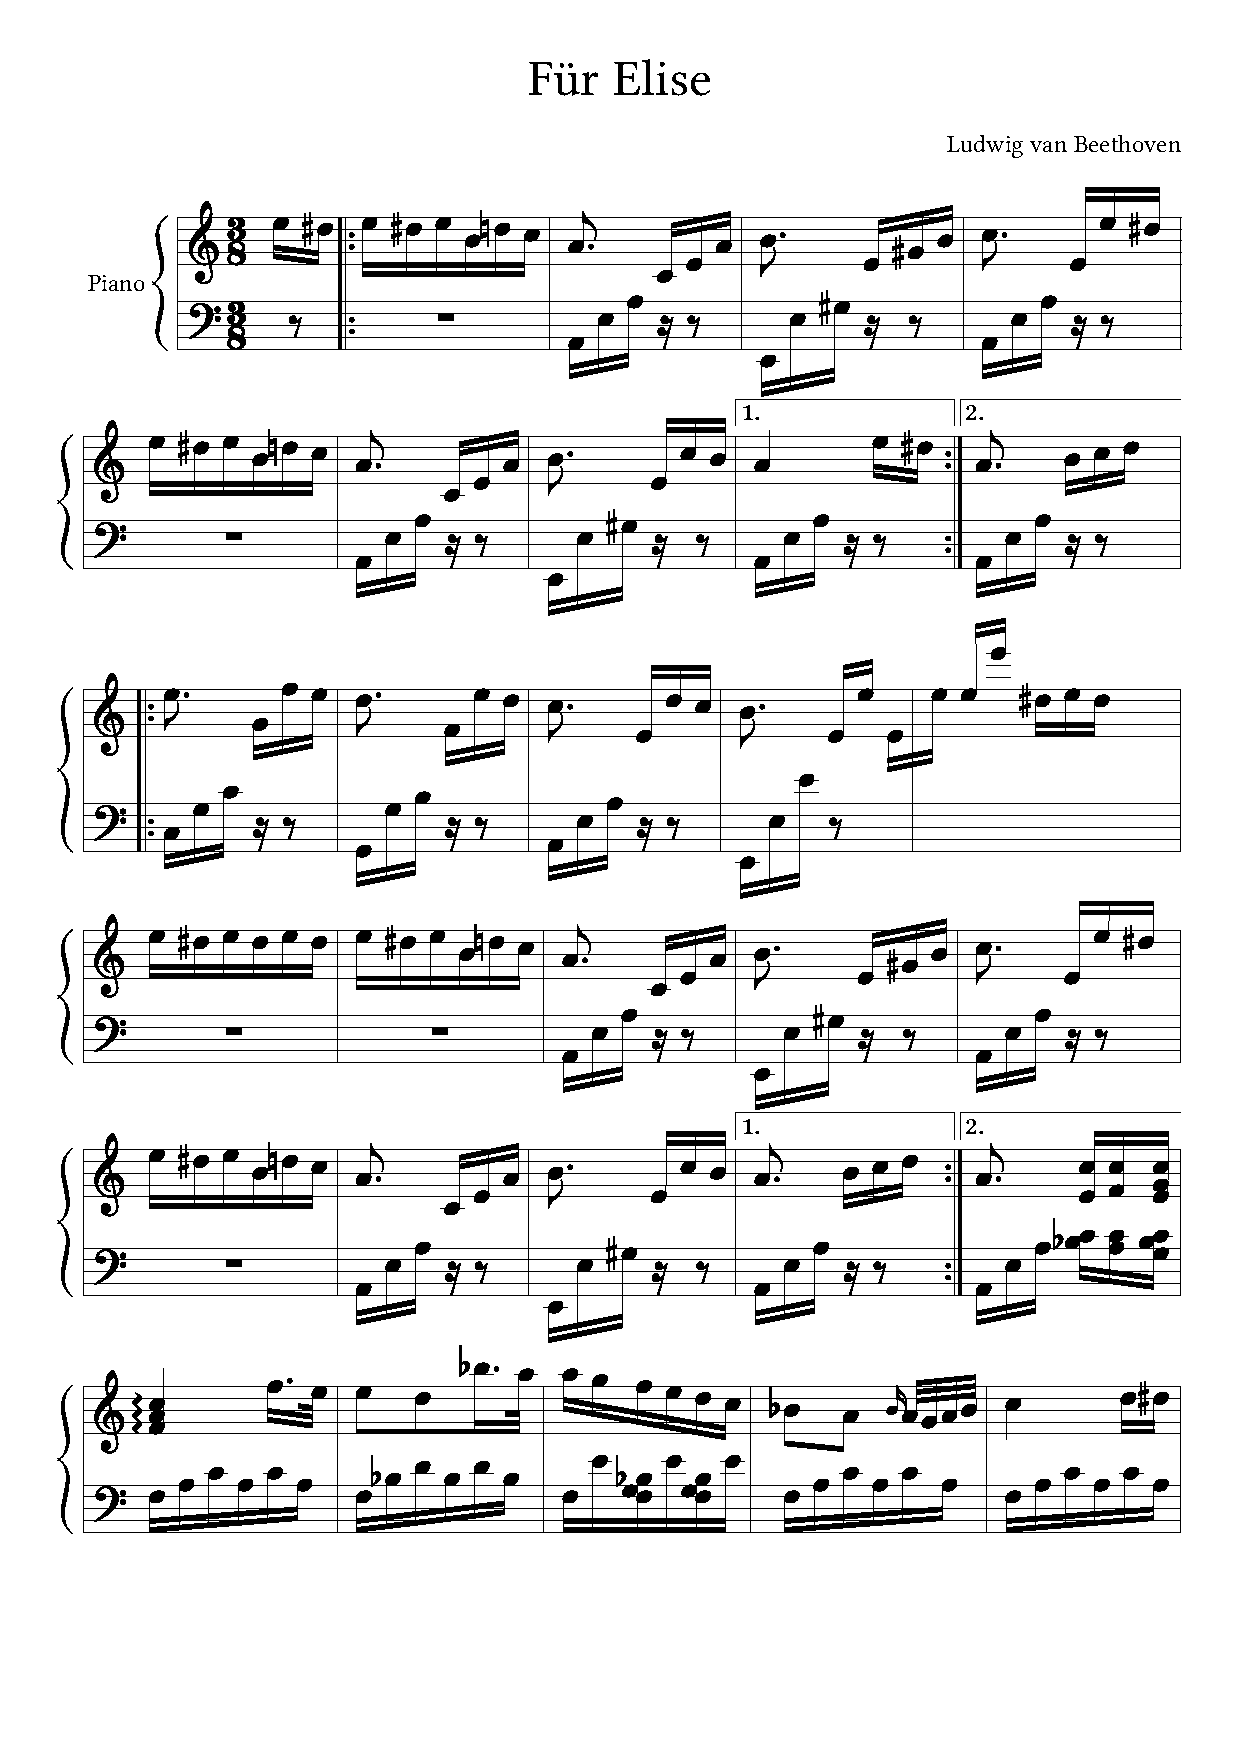
\includepdf{demo/demo-1.pdf}